\subsubsection{Coherence Block}\label{subsec:bloco-coerencia}
The frequency interval over which the channel remains approximately constant is called the Coherence Bandwidth ($B_c$). A coherence block is a region with duration $T_c$ and bandwidth $B_c$. Within the coherence block, the effect of the channel on the signal is the same as multiplying by a complex gain \cite{marzetta2016fundamentals} (Figure~\ref{fig:bloco-coerencia}). \textcolor{blue}{This work uses $B_c = 1$ PRB \cite{zhao2025jsac}.}
The number of OFDM symbols in a coherence block is limited by $T_c$. \textcolor{blue}{Table~\ref{tab:n-maximo} shows how many OFDM symbols fit within $T_c$ for each test condition, with subcarrier spacings of 30 kHz (FR1) and 120 kHz (FR2) \cite{3gpp-ts38104}.}

% FONTE: SCS: TS 38.104 Tab. 5.3.5-1 (n78) e 5.3.5-2 (n257).
% FONTE: Marzetta et al., Seções 2.1.2 e 2.1.3, pp. 21-22.
\begin{figure}[!ht]
\caption{Time-frequency plane divided into coherence blocks.}
\label{fig:bloco-coerencia}
\vspace{4pt}
\centering
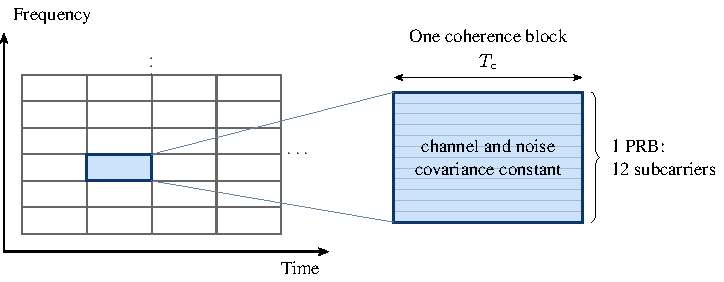
\includegraphics{Images/FLUXO/bloco_coerencia.pdf}
\vspace{4pt}
\legend{Source: adapted from \citesp{bjornson-mimo}.}
\end{figure}
% FONTE: zhao2025jsac (canal constante no PRB). Figura: Björnson et al., Fig. 2.1, p. 67.

